\documentclass[11pt,a4paper]{article}
\usepackage{termpaper}
\usepackage[utf8]{inputenc}
\usepackage{mathtools}
\usepackage{tabularx}
\usepackage{graphicx}

\newtheorem{definition}{Definition}
\DeclarePairedDelimiter\norm{\lVert}{\rVert}
\newcolumntype{Y}{>{\centering\arraybackslash}X}
%opening
\title{Clustering with Affinity Propagation and its Applications}
\author{
 \authorname{Philipp-Alexander Auer} \\
 \studentnumber{01420446} \\
 \curriculum{033 535} \\
 \email{e1420446@student.tuwien.ac.at}
}

\begin{document}

\maketitle

\begin{abstract}
When working on data-sets a crucial step is often to cluster the data points. To do so, clustering algorithms such as k-means were developed. In 2007 Frey et al. introduced Affinity Propagation \cite{frey2007clustering} a message-passing based clustering algorithm, that can work on arbitrary data sets without knowing the number of clusters beforehand, given a similarity criterion. Researchers have since improved Affinity Propagation to improve its convergence behavior \cite{wang2008adaptive} and applied it to different real-life scenarios, such as position tracking in wireless local area networks. \cite{tian2013fingerprint}
\end{abstract}

\section{Introduction}

Finding groups in data is an important step in many fields of computer science, and already there exist algorithms to solve these problems. One solution to this is the popular k-means, or k-centers algorithm, which iteratively refines a randomly selected initial set of clusters. This method comes with the constraint that a user has to specify the initial amount of clusters, and is very sensitive to that parameter. \cite{frey2007clustering} 
Affinity Propagation is a clustering algorithm proposed by Frey et al. in 2007. It uses a message passing model between data points to form a collection of exemplars (See Definition \ref{def:exemplar}) and respective clusters. \cite{frey2007clustering} Affinity Propagation tries to solve the problem without needing to know the number of clusters beforehand, by only supplying a similarity criterion.
While the proposed method performs better for many tested applications \cite{frey2007clustering} and has very good general applicability, there are a number of problems that occur when strictly following the procedure, one of them being numerical oscillations in the message passing procedure. Wang et al. try to tackle this with their adaptive version of the algorithm, which changes parameters on the fly, to achieve better results and convergence times. \cite{wang2008adaptive} With the original implementation of Affinity Propagation and some further improvements, the procedure promises to be a valid applicant to tackle modern problems that require a form of uninformed clustering on different data sets. Tian et al. propose a probability distribution-aided algorithm to perform fingerprint indoor positioning in WLAN networks, which is based on an initial Affinity Propagation Clustering. Their results outperformed other algorithms in performance and accuracy. \cite{tian2013fingerprint}

\begin{definition}\label{def:exemplar}
	An exemplar is a data point that is selected as the center of a cluster.
\end{definition}

\pagebreak
\section{Affinity Propagation}

Affinity Propagation works by passing messages between individual nodes in order to cumulative evidence of responsibility and availability. The input parameter is the similarity of all nodes. This information is stored in matrices. (See Definition \ref{def:matrices}) Each entry of such a matrix encodes information about point $x_i$ and $x_k$ in the data set. Affinity Propagation can be used to identify clusters, and their respective exemplars.
\begin{definition}\label{def:matrices}
	Matrices used in the Affinity Propagation Algorithm
	\[
		\mathsf{Similarity\ Matrix:}\  S(i,k) 
	\]
	\[
		\mathsf{Responsibility\ Matrix:}\  R(i,k) 
	\]
	\[
		\mathsf{Availability\ Matrix:}\  A(i,k) 
	\]
\end{definition}
\subsection{Similarity}
When talking about clusters an understanding of similarity is needed. Affinity Propagation gets this from $S(i,k)$. This general parameter encodes how suited $x_k$ is to be an exemplar for point $x_i$. Metrics prove to be a good similarity criterion, so as a default the negative squared error can be used as input for the similarity matrix. \cite{frey2007clustering} (See Definition \ref{def:negsquared}) It is important to note that $S$ can take any real values, and if another exemplar-based probability model is available, $S(i,k)$ can be set to the real-valued log-likelihood of $x_i$, given that its exemplar is $x_k$. This correlation is not necessarily symmetric, and can be set by hand if needed. \cite{frey2007clustering}
\begin{definition}\label{def:negsquared}
	Negative squared error (euclidean distance)
	\[
		S(i,k) = - \norm{x_i - x_k}^2
	\]
\end{definition}
Additionally, the diagonal values $S(k,k)$ of the similarity matrix are special, as they represent how likely it is for $x_k$ to be an exemplar itself. Those values $p_1 .. p_n$ are called preference values:
\[
	S(i,k) = \begin{bmatrix}p_{1} & & \\ & \ddots & \\ & & p_{n}\end{bmatrix}
\]
Rather than requiring the a priori knowledge about the number of clusters, they emerge from those preference values, and the later explained message passing procedure. If each point is equally likely to be an exemplar, the preference values can be set to a common value $p_1..p_n = p$. A higher preference will yield more clusters, so for a moderate amount, $p$ can be set to the median of all similarities. For a small amount it can be set to the minimum. \cite{frey2007clustering}

\subsection{Responsibility}
One of the two exchanged messages is the so-called responsibility $R(i,k)$, sent from $x_i$ to $x_k$. It reflects the accumulated evidence for how well-suited point $x_k$ is to serve as the exemplar for point $x_i$, taking into account other potential exemplars for point $x_i$. \cite{frey2007clustering}
\subsection{Availability}
The other exchanged message is called availability $A(i,k)$, sent from $x_k$ to $x_i$. It reflects the accumulated evidence for how appropriate it would be for point $x_i$ to choose point $x_k$ as its exemplar, taking into account the support from other points that point $x_k$ should be an exemplar. Both Responsibility and Availability can be viewed as log-probability ratios. To initialize the algorithm $A$ is set to $A(i,k) = 0$. \cite{frey2007clustering}
\pagebreak
\subsection{Passing Messages}
Both $R$ and $A$ serve as message-passing matrices. The actual message exchange is modelled by applying update rules to $R$ and $A$. First, the responsibility is updated according to Definition \ref{def:respupdate}, then the new availability is calculated according to Definition \ref{def:avupdate}.
\begin{definition}\label{def:respupdate}
	Updating the Responsibility
	\[
		R(i,k) \leftarrow S(i,k) - \underset{k^\prime\, \mathsf{s.t.}\, k^\prime \neq k}{\mathsf{max}} \{A(i,k^\prime) + S(i,k^\prime)\}
	\]
\end{definition}
\begin{definition}\label{def:avupdate}
	Updating the Availability
	\[
		A(i,k) \leftarrow \mathsf{min}\{0,R(k,k) + \sum\limits_{i^\prime\,\mathsf{s.t.}\, i^\prime \notin \{i,k\}}\mathsf{max}\{0, R(i^{\, \prime} ,k)\}\}
	\]
\end{definition}
As points get effectively assigned to an exemplar, their availability will drop below 0, weakening the incoming positive values from the initial similarity. $R(k,k)$, the "Self-Responsibility" can be interpreted as accumulated evidence, that $x_k$ is an exemplar, based on its preference, and how ill-suited it is to serve as an exemplar for other points. \cite{frey2007clustering} While the responsibility updates let candidate exemplars compete for the ownership of a data point, the availability updates gather evidence whether a candidate exemplar would be a good one. It is noteworthy that only positive responsibilities are accounted for, because a good exemplar only needs to explain some data points well, regardless of how poorly it explains others. \cite{frey2007clustering} The "Self-Availability" $A(k,k)$ reflects accumulated evidence that $x_k$ is an exemplar, based on positive responsibilities sent to it from other points. It needs its own update rule (See Definition \ref{def:savupdate})
\begin{definition}\label{def:savupdate}
	Updating the "Self-Availability"
	\[
   		A(k,k) \leftarrow \sum\limits_{i^\prime\, \mathsf{s.t.}\, i^\prime \neq k} \mathsf{max} \{0, R(i^{\, \prime} ,k)\}
	\]
\end{definition}
All of the update rules can be done with simple, local computations. \cite{frey2007clustering}
\subsection{Retrieving Data}
At any point during the iterative process, $A$ and $R$ can be combined to identify exemplars. For $x_i$, the $x_k$ maximizing
\[
	A(i,k) + R(i,k)
\]
either identifies $x_i$ as an exemplar if $i=k$ or $x_k$ as an exemplar for $x_i$. \cite{frey2007clustering} For reasonable results the algorithm may be terminated after a fixed number of iterations, after changes in messages fall below a a threshold, or after the local decisions stay constant for some number of iterations. \cite{frey2007clustering}

A visualized form of the message-passing procedure can be seen in Figure \ref{fig:iterations}, where you can see how each point gradually chooses its exemplar.
\begin{figure}[h!]
	\centering
	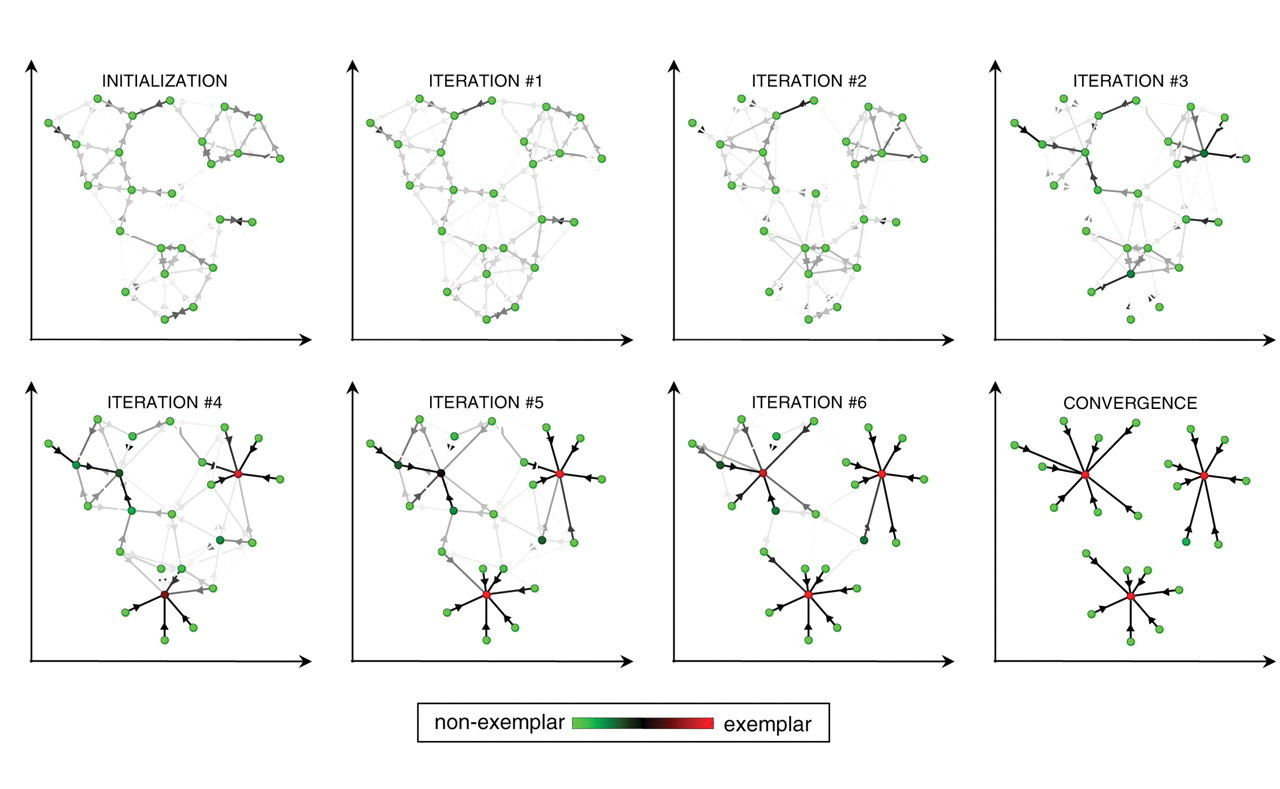
\includegraphics[width=\textwidth]{../figures/frey-dueck-cluster.jpg}
	\caption{Visualized message-passing procedure \cite{frey2007clustering} showing the likelihood of a point being an exemplar, and its exemplar-relation to other points.}
	\label{fig:iterations}
\end{figure}
\pagebreak
\subsection{Numerical Oscillations}
When passing the messages, numerical oscillations may occur in the matrices. To tackle them, messages must be damped. This is done using a damping factor $\lambda \in \left[0,1\right]$ and applied to each message update. Such a damped message-pass follows Definition \ref{def:dampupdate}. The damping factor may be chosen freely in the interval $[0,1]$, a default value of $\lambda = 0.5$ is specified by Frey et al. \cite{frey2007clustering}
\begin{definition}\label{def:dampupdate}
	Updating message matrix $M$ using damping factor $\lambda$
	\[
		M^\prime (i,k) =\lambda \cdot M_{\mathsf{old}}(i,k) + (1-\lambda) \cdot M_{\mathsf{new}} (i,k)
	\]
\end{definition}
It is to note that a high damping factor can get rid of oscillations well, but it may slow down the message passing procedure. \cite{wang2008adaptive} Finding an appropriate damping factor is not trivial, Wang et al. propose their Adaptive Affinity Propagation algorithm in order to tackle that, among other things. \cite{wang2008adaptive}
\pagebreak
\subsection{Advantages}
As already mentioned, clusters and exemplars in Affinity Propagation emerge out of the preference values and message-passing process naturally. It is not required to supply the dedicated number of expected clusters like for e.g. k-centers clustering. \cite{frey2007clustering}

Additionally Affinity Propagation can also operate on unusual, non-metric spaces. The similarity matrix does not need to be symmetric (See Definition \ref{def:symmetric}), and the similarities do not have to satisfy the triangle inequality. (See Definition \ref{def:triangleieq}) \cite{frey2007clustering}

Given that, Affinity Propagation is in some senses more versatile than classical approaches. An example where those (missing) constraints are used was conducted by Frey et al. in \cite{frey2007clustering} where they tried to cluster sentences, with similarity $S(i,k)$ based on the cost of encoding words in sentence $i$ with words of sentence $k$. 97\% of the resulting similarities where non-symmetric. \cite{frey2007clustering} 
\begin{definition}\label{def:symmetric}
	Similarities do not have to be symmetric: $S(i,k) = S(k,i)$.
\end{definition}
\begin{definition}\label{def:triangleieq}
	Similarities do not have to satisfy the triangle inequality: $S(i,k) < S(i,j) + S(j,k)$
\end{definition}
\subsection{Results}
Frey et al. conducted a series of experiments to compare Affinity Propagation to k-centers clustering. For a complete list see \cite{frey2007clustering}.
\subsubsection{Face Images}
A classic problem is image clustering. To study this, Affinity Propagation was applied on 900 grey-scale images of faces. The results show, that even after a large amount of re-runs Affinity Propagation has a lower squared error, compared to k-centers clustering. Affinity Propagation uniformly achieved a much lower error in more than two orders of magnitude less time. \cite{frey2007clustering}

When using a different error metric on this problem, namely absolute pixel distance, Affinity Propagation also uniformly outperformed k-centers clustering. \cite{frey2007clustering}
\subsubsection{Clustering Putative Exons}
When trying to find genes, clustering of putative exons plays a huge role. \cite{frey2007clustering} It is interesting to see how Affinity Propagation performs here, because the similarity matrix derived from mined DNA sequences is sparse. In this task one run of Affinity Propagation was run once and took 6 minutes, while 10.000 runs of k-centers clustering took 208 hours. The results show a high True Positive rate of 39\% at a False Positive rate of 3\%. k-centers did not nearly perform as well, at only a TP rate of 17\%. It is to note that a more sophisticated tool with additional biological knowledge could achieve a TP rate of 43\% at the same FP rate. \cite{frey2007clustering}
\pagebreak
\section{Adaptive Affinity Propagation}
As already mentioned, the message-passing process in Affinity Propagation can lead to numerical oscillations, which cannot be eliminated automatically. Choosing a high value for the damping factor $\lambda$, will indeed get rid of oscillations in most cases, but also slows down the message-passing part of the algorithm. Additionally, optimal preference values depend not only on measures of similarity, but also the structure of the data set, and the desired outcome. While the median of all similarities is a good value for a common preference value $p$, it does not account for said factors. Wang et al. propose their "adaptive" version of the Affinity Propagation algorithm, in order to overcome the limitations of numerical oscillations, and adaptively change both the damping factor $\lambda$ and the preference value $p$. \cite{wang2008adaptive}

Adaptive AP proposes methods to adaptively change the damping factor in order to eliminate oscillations (Adaptive Damping), to adaptively change the preference values to escape oscillations if that fails (Adaptive Escape) and adaptively searching the space of $p$ to find an optimal clustering solution suitable for the data set (Adaptive Preference scanning)
\subsection{Overcoming numerical oscillations}
A trivial solution to get rid of oscillations and achieve convergence is to use a high damping factor ($\lambda$ close to $1$), which will cause the algorithm to converge, but run very slow. \cite{wang2008adaptive}

Another solution is to re-run AP with different damping factors if the model fails to converge in the beginning. That requires to repeat the whole message-passing part many times, and will also consume a lot of time and resources. \cite{wang2008adaptive}

\subsubsection{Adaptive Damping}
The proposed method scans for occurrences of non-oscillating features (See Definition \ref{def:nonosc}) in a sliding window of size $w$. (Because detecting oscillations is generally harder, than detecting those non-oscillating features) If oscillations are detected, $\lambda$ is increased by a step (e.g. $\lambda_\Delta = 0.05$). If the number of non-oscillating features is less than two-thirds of the window size, oscillations are detected. This is a tolerant design and accounts for occasional vibrations, as well as initial oscillations in the first iterations. \cite{wang2008adaptive} If this technique fails to get rid of the oscillations and $\lambda$ reaches a threshold (e.g. $\lambda_{\mathsf{max}} = 0.85$) it means that the adaptive damping failed, and $p$ is changed instead, in the Adaptive Escape method described below.
\begin{definition}\label{def:nonosc}
	Non-Oscillating feature: The number of exemplars is decreasing or unchanged in the iterative process. \cite{wang2008adaptive}
\end{definition}
\subsubsection{Adaptive Escape}
When adaptive damping alone fails, another way to escape oscillations is to decrease $p$, which will yield less clusters and eliminate oscillations according to Definition \ref{def:nonosc}. The adaptive escape is used when $\lambda$ reaches its threshold $\lambda_{\mathsf{max}}$, and decreases the preference value $p$ by $p_{\Delta}$. \cite{wang2008adaptive} This is used in combination with the Adaptive Preference Scanning technique described below.
\subsection{Adaptive Preference Scanning}
Additionally, the new proposed method is able to search through different values of $p$ in order to find better solutions. This requires to adaptively adjust $p$ throughout the algorithm, to obtain different results. Those are then compared using the silhouette index \cite{ROUSSEEUW198753} as a validity index. It is crucial for both performance and results, that step sizes for $p$, as well as window sizes are chosen accordingly. Wang et al. derived reasonable limits and default values for all of those in \cite{wang2008adaptive}.
\pagebreak
\subsection{Results}
The following table (Table \ref{tbl:adapres}) shows a comparison between Affinity Propagation (AP) and adaptive Affinity Propagation (adAP). The results show that adAP performs better and comes closer to the actual know cluster numbers. It can indeed eliminate oscillations when they occur. One can also see, that the additional escape and scanning techniques do contribute a significant time overhead, which is a trade off in order to achieve better results. Table \ref{tbl:adapres} also shows that adaptive Affinity Propagation performs best compared to regular AP when it is able to detect and eliminate oscillations.
\begin{table}[h]
	\begin{center}
		\begin{tabularx}{\textwidth}{@{}XYYYYYYYYY@{}}
			\hline
			Data sets&known NC  &adAP NC  &adAP error (\%) & adAP FM  &adAP time(s) & adAP eliminate oscillations  & AP NC  & AP FM  & AP time(s)  \\\hline
			3k2lap&3  &3  &7.67  &0.85  &144.0  &/  &16  &0.39  &2.1  \\
			5k8close&5  &5  &0  &1.00  &1851.0  &/  &17  &0.56  &31.2  \\
			14k10close&14  &14  &0  &1.00  &275.5  &/  &15  &0.97  &6.0  \\
			22k10far&22  &22  &0  &1.00  &1125.9  &yes  &168  &0.80  &307.8  \\
			Ionosphere&2  &2  &17.4  &0.75  &445.3  &yes  &28  &0.47  &56.8  \\
			Wine&3  &3  &10.7  &0.80  &34.5  &/  &11  &0.46  &0.5  \\
			Yeast&4  &4  &3.37  &0.97  &54.7  &/  &11  &0.66  &0.9  \\
			NCI60&8  &8  &/  &0.56  &12.9  &/  &9  &0.48  &0.1  \\
			FaceImage&100  &102  &/  &/  &3701.2  &/  &103  &/  &14.5  \\
			Document&4  &4  &/  &/  &0.3  &/  &4  &/  &0.2  \\
			Travelroute&7  &7  &/  &/  &24.7  &/  &7  &/  &20.0  \\
			Exons&/  &102  &/  &32.8\%  &83073.7  &/  &37  &22.4\%  &996.0\\\hline 
		\end{tabularx}
	\end{center}
	
	\caption{Clustering results of adAP and AP \cite{wang2008adaptive}}
	\label{tbl:adapres}
\end{table}
\pagebreak
\section{Application: Fingerprint indoor positioning}
Several approaches exist for tracking the position of a user in a wireless local area network. They take into account measurements like time of arrival, angle of arrival, and received signal strength of radio waves in the communication. Of those, only the received signal strength (RSS) is suitable for usage when you do not have the necessary hardware to also track the other factors. Positioning based on RSS, however, comes with some challenges, mostly because of irregular variations in the RSS. \cite{tian2013fingerprint}

Tian et al. propose an algorithm based on RSS readings. To do so, they construct and cluster a radio map in the so-called Off-line phase, and use a 2-step model to calculate the users position by first estimating a cluster (Coarse Positioning), and later calculating the coordinates (Fine Positioning). \cite{tian2013fingerprint}
\subsection{Building the radio map}
RSS readings are measured at specific reference points (RP) for the access points (AP). The results are averaged and stored. The value measured at $\mathsf{RP}_j$ for $\mathsf{AP}_i$ is called $\Psi_{i,j}$. All of the values can be stored in a matrix $\Psi$ and are called the radio map \cite{tian2013fingerprint}:
\[\Psi = 
\left( \begin{array}{cccc}
\Psi_{1,1} & \Psi_{1,2} & \dots & \Psi_{1,N} \\                                              
\Psi_{2,1} & \Psi_{2,2} & \dots & \Psi_{2,N} \\
\vdots & \vdots & \ddots & \vdots \\
\Psi_{L,1} & \Psi_{L,2} & \dots & \Psi_{L,N} \\                                        
\end{array}\right)
\]
Clustering is a crucial step of the proposed algorithm, because it helps to mitigate the degradation of accuracy and is beneficial to reduce the computation cost since only the cluster centers are considered for the positioning. \cite{tian2013fingerprint}

The similarity matrix required for AP is calculated using the column vectors of the radio map
\[
\vec{\Psi}_j = \left[\Psi_{1,j}, \Psi_{2,j}, \dots , \Psi_{L,j}\right]^T, j=1,2,\dots , N
\]
with the negative squared error:
\[
S(i,j) = -\norm{\vec{\Psi}_i - \vec{\Psi}_j}^2, \forall i,j \in \{ 1,2,\dots , N \}
\]

Affinity Propagation is run as described in the above sections, and the cluster exemplars are used as reference points for the tracking algorithm. \cite{tian2013fingerprint}
\subsection{Results}
Tian et al. compared their proposed algorithm to Knn. They also tried to apply clustering to Knn. Clustering was tested with k-means and Affinity Propagation. They also tried their probability based method with k-means instead of Affinity Propagation. Results can be seen in Table \ref{tbl:fingerprint}
\begin{table}[h]
	\begin{center}
		\begin{tabularx}{\textwidth}{@{}XYYY@{}}
			\hline
			Algorithm & Mean ($m$) & Max ($m$) & Variance ($m^2$)\\\hline
			K-means + Knn & 3.38 & 6.72 & 2.82\\
			K-means + Probability Distribution & 3.11 & 6.70 & 3.24\\
			Affinity Propagation + Knn & 2.66 & 6.67 & 3.02 \\
			Proposed Algorithm & 2.23 & 6.52 & 2.52\\
			\hline
		\end{tabularx}
	\end{center}
	\caption{Results of statistical positioning errors \cite{tian2013fingerprint}}
	\label{tbl:fingerprint}
\end{table}

As you can see from the experimental results, Affinity Propagation increases the performance for both Knn and the Probability Distribution based method proposed by Tian et al.
\section{Conclusion}
Since it was introduced by Frey et al. in 2007, Affinity Propagation has been applied successfully to different projects. The new method increased performance while lowering computational cost compared to conventional methods. Researchers have adapted the algorithm to further improve its performance. Clustering is often a crucial step when preprocessing data sets for further applications, having a method with general applicability and performance has already lead to improvement in research, and will be beneficial in the future.
\bibliographystyle{plain}
\bibliography{../literature/literature}

\end{document}
